\documentclass[degree=doctor,secret]{cugthesis}
% 选项:
%   degree=[bachelor|master|doctor|postdoctor], % 必选
%   secret,                                       % 可选
%   pifootnote,                                 % 可选(建议打开)
%   openany|openright,                	  % 可选,基本不用
%   arial,                                      	% 可选,基本不用
%   arialtoc,                                     % 可选,基本不用
%   arialtitle                                     % 可选,基本不用

% 所有其它可能用到的包都统一放到这里了,可以根据自己的实际添加或者删除。
\usepackage{threeparttable} %三线表,带表注释

%**************************一些使用量很高的变量定义**********************************
%\def\ca{{\text{Ca}^{2+}}}   			%公式: 使用时必须放在$$内当公式用
%****************************************************************************************

% 定义所有的图片文件在 figures 子目录下
\graphicspath{{figures/}{../../figures/}}

% 可以在这里修改配置文件中的定义。导言区可以使用中文。
\begin{document}

%%% 封面部分
\frontmatter
\thusetup{
	%******************************
	% 注意:
	%   1. 配置里面不要出现空行
	%   2. 不需要的配置信息可以删除
	%******************************
	%
	%=====
	% 秘级
	%=====
	secretlevel={秘密},
	secretyear={10},
	%
	%=========
	% 中文信息
	%=========
	ctitle={ xxxx热液xxxxxx研究},
	cdegree={理学博士},
	cuniversity={中国地质大学},
	euniversity={China University of Geosciences},
	cdepartment={地球物理与空间信息学院},
	cmajor={地球物理学},
	cauthor={郭志馗},
	studentnum={22015xxxxx},
	csupervisor={xx教授},
	cassosupervisor={xxx研究员}, % 副指导老师
	ccosupervisor={xx Rüpke 教授}, % 联合指导老师
	cproject={国家留学基金委},
	% 日期自动使用当前时间,若需指定按如下方式修改:
	% cdate={超新星纪元},
	%
	% 博士后专有部分
	cfirstdiscipline={计算机科学与技术},
	cseconddiscipline={系统结构},
	postdoctordate={2009年7月——2011年7月},
	id={编号}, % 可以留空: id={},
	udc={UDC}, % 可以留空
	catalognumber={分类号}, % 可以留空
	%
	%=========
	% 英文信息
	%=========
	etitle={Numerical simulation xxxxxx},
	% 这块比较复杂,需要分情况讨论:
	% 1. 学术型硕士
	%    edegree:必须为Master of Arts或Master of Science(注意大小写)
	%             “哲学、文学、历史学、法学、教育学、艺术学门类,公共管理学科
	%              填写Master of Arts,其它填写Master of Science”
	%    emajor:“获得一级学科授权的学科填写一级学科名称,其它填写二级学科名称”
	% 2. 专业型硕士
	%    edegree:“填写专业学位英文名称全称”
	%    emajor:“工程硕士填写工程领域,其它专业学位不填写此项”
	% 3. 学术型博士
	%    edegree:Doctor of Philosophy(注意大小写)
	%    emajor:“获得一级学科授权的学科填写一级学科名称,其它填写二级学科名称”
	% 4. 专业型博士
	%    edegree:“填写专业学位英文名称全称”
	%    emajor:不填写此项
	edegree={Science},
	emajor={Geophysics},
	eauthor={Zhikui Guo},
	esupervisor={Prof. Dr. xx},
	eassosupervisor={Prof. Dr. xx },
	ecosupervisor={Prof. Dr. xx xx},
	eaddress={Wuhan 430074 P.R. China},
	% 日期自动生成,若需指定按如下方式修改:
	% edate={December, 2005}
	%
	% 关键词用“英文逗号”分割
	ckeywords={\TeX, \LaTeX, CJK, 模板, 论文},
	ekeywords={\TeX, \LaTeX, CJK, template, thesis}
}

% 定义中英文摘要和关键字
\begin{cabstract}
	论文的摘要是对论文研究内容和成果的高度概括。摘要应对论文所研究的问题及其研究目
	的进行描述,对研究方法和过程进行简单介绍,对研究成果和所得结论进行概括。摘要应
	具有独立性和自明性,其内容应包含与论文全文同等量的主要信息。使读者即使不阅读全
	文,通过摘要就能了解论文的总体内容和主要成果。
	
	论文摘要的书写应力求精确、简明。切忌写成对论文书写内容进行提要的形式,尤其要避
	免“第 1 章……;第 2 章……;……”这种或类似的陈述方式。
	
	本文介绍中国地质大学(武汉)论文模板 \thuthesis{} 的使用方法。本模板符合学校的本科、硕士、
	博士论文格式要求。
	
	本文的创新点主要有:
	\begin{itemize}
		\item 用例子来解释模板的使用方法;
		\item 用废话来填充无关紧要的部分;
		\item 一边学习摸索一边编写新代码。
	\end{itemize}
	
	关键词是为了文献标引工作、用以表示全文主要内容信息的单词或术语。关键词不超过 5
	个,每个关键词中间用分号分隔。(模板作者注:关键词分隔符不用考虑,模板会自动处
	理。英文关键词同理。)
\end{cabstract}

% 如果习惯关键字跟在摘要文字后面,可以用直接命令来设置,如下:
% \ckeywords{\TeX, \LaTeX, CJK, 模板, 论文}

\begin{eabstract}
	An abstract of a dissertation is a summary and extraction of research work
	and contributions. Included in an abstract should be description of research
	topic and research objective, brief introduction to methodology and research
	process, and summarization of conclusion and contributions of the
	research. An abstract should be characterized by independence and clarity and
	carry identical information with the dissertation. It should be such that the
	general idea and major contributions of the dissertation are conveyed without
	reading the dissertation.
	
	An abstract should be concise and to the point. It is a misunderstanding to
	make an abstract an outline of the dissertation and words ``the first
	chapter'', ``the second chapter'' and the like should be avoided in the
	abstract.
	
	Key words are terms used in a dissertation for indexing, reflecting core
	information of the dissertation. An abstract may contain a maximum of 5 key
	words, with semi-colons used in between to separate one another.
\end{eabstract}

% \ekeywords{\TeX, \LaTeX, CJK, template, thesis}

% 如果使用授权说明扫描页,将可选参数中指定为扫描得到的 PDF 文件名,例如:
% \makecover[scan-auth.pdf]
\makecover

%% 目录
\tableofcontents

%% 符号对照表
%\begin{denotation}[3cm]
\item[HPC] 高性能计算 (High Performance Computing)
\label{denotation0}
\end{denotation}


%%% 正文部分
\mainmatter

\chapter{绪论}
\label{chapter:Introduction}

本章主要展示章-节-小节格式。

\section{研究背景、目的和意义}
学位论文,尤其是博士学位论文少则一百多页,多则超过两百页。
如此长篇的论文如果用word编写,则会遇到很多问题。
首先是排版问题:文本字体、段落格式、行内公式、行间公式、参考文献引用、图表交叉引用等,
用word做这类事情真是一种煎熬(只是个人感受)。
但是latex可轻松搞定这一切,只需将所有注意力放在内容创作上即可。
其次是加载图片问题,首先word无法插入高分辨率的矢量图,而且文档中图片很多的时候整个操作会很卡。
而latex只需要将所有的图片放在指定的目录里面,然后在使用的地方用一句简单的命令包含进来即可,并不会影响latex文档大小。
这只是在此提到的两个主要问题,相信写过或者正在写学位论文的同学才能真正明白其中的苦衷。

本模板CugThesis latex模板是作者自己根据ThuThesis模板和中国地质大学(武汉)学位论文编写规范制定的。
以方面方便自己的博士论文编写,另一方面可以将其分享给地大的学子们,当然了是有兴趣用latex编写论文的同学!
但在此申明:作者只是分享而已,根据自己情况选择,作者不对使用此模板导致的任何问题负责任!


\section{研究现状和存在问题}


\subsection{国内外研究现状和发展趋势}
在国外很多大学都有其学位论文latex模板,而且大多数大学都建议毕业生用latex编写 学位论文 \citep{andersen2017faulting}。
而国内虽然大多数大学没有这么建议,但是也已经有不少大学的毕业生自己制作latex模板 ,并在网络上分享。比如清华大学、中国科学技术大学、南京大学等。
对于中国地质大学(武汉)的学位论文latex模板,之前有地空学院的一位学长做过latex模板,
但是本人并没有测试成功(可能是本人对齐设置有误等原因),也有计算机学院等同学做了相应的模板。


\subsection{存在问题和发展趋势}
latex编写论文,唯一的缺点就是审阅模式问题。
这也是latex写作很难推广的一个主要原因,
与word审阅模式不同 ,latex主流的免费编辑器(比如TeXstudio并不支持审阅模式)。
所以如果导师非要用 word审阅模式的方式来修改论文,那么这种方式就是个很大的问题。
否则,用latex写学位论文只有高效和稳定,尤其是再用git进行 版本控制!

参考文献使用实例: \cite{coumou2006dynamics}研究了海底热液系统的三维模拟。




\chapter{模板使用方法}

对于一篇毕业论文,基于latex写作的时候,我们需要关注的就是如何插入图片、文献、表格、公式以及如何交叉引用。主要就是这几点,当然还有一些细节性的东西,作者会持续更新到 \href{https://www.jianshu.com/p/c9bb775fe0f4}{简书文章: CugTheis使用说明}  里面。

\subsection{插入图片}
\begin{figure} [htbp] 
	\centering
	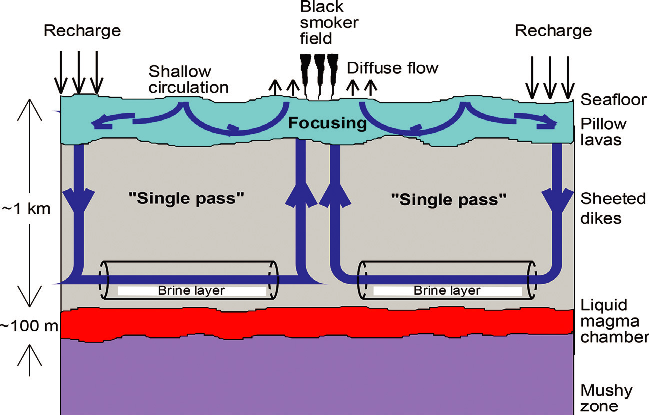
\includegraphics[width=\textwidth ]{SinglePassModel} 
	\caption[单通道模型]{Single Pass Model} 
	\fnote{海底热液循环系统示意图,包含了recharge区域和discharge区域。海水被岩浆热源加热后在深部发生 相分离,分离为密度较大的卤水(液相)和密度较小的蒸汽相,向上浮动。\textcolor{green}{这是一个但排列图}} 
	\label{fig:singlepassmodel} 
\end{figure} 

 \autoref{fig:singlepassmodel} 是一个单排列图\footnote{这是个脚注:注意这里的参考文献引用}
  \citep{andersen2017faulting}。每个图可根据实际意义命名一个label,方便后面进行交叉引用。
  caption设置是必须的,表示这个图的标题。如果此图有一段图注的话,使用fnote来设置。看 \autoref{fig:singlepassmodel} 的latex代码。为了生成图和表的索引,在图和表的caption前面也可以用方括号设置其shor-caption用于后面的图和表索引标题显示,比如  \autoref{fig:singlepassmodel} 的\textbf{单通道模型} 短标题。


\begin{figure} [htbp]
	\centering%
	\subcaptionbox{CUG彩色logo\label{fig:cug1} }  
	{
\includegraphics[height=0.3\textwidth]{CUG_Logo1} } 
	\hspace{0.01\textwidth} 
	\subcaptionbox{微信公众号\label{fig:weixin} }  
	{
\includegraphics[height=0.3\textwidth]{weixingongzhong} } 
		\hspace{0.01\textwidth} 
	\subcaptionbox{CUG黑白logo\label{fig:cug2} }  
	{
\includegraphics[height=0.3\textwidth]{CUG_Logo2} } 
	\caption{三列图示例} 
	\label{fig:figure_3col} 
\end{figure} 

\autoref{fig:figure_3col} 是一个三列子图示例,总图有编号和标题。每个子图也有相应的编号和标题,也可以交叉引用其中一个子图,比如 扫码 \ref{fig:weixin} 关注微信公众号获取更多学术资源!


\subsection{表格}

本模板支持三线表比如

\begin{table}[htbp]
	\centering
	\caption{数学符号和物理意义列表}
	\label{tab:symbols_values}
	\begin{tabular}{cccc}
		\toprule 
		数学符号 & 物理意义 & 典型取值 &单位 \\
		\midrule
		$\vec{g}$ & 重力加速度矢量 & 9.8 & $m/s^2$ \\
		$\rho_f$ & 水的密度 & 1.0 & $kg/m^3$ \\
		\bottomrule
	\end{tabular}
\end{table}

\autoref{tab:symbols_values} 是一个三线表,有其标题和label(用于交叉引用)。

\subsection{公式}

行内公式,这个是行内公式 $E=MC^2$,下面是个带编号的独立公式:

\begin{equation}
\left( {\phi {\rho _f}{c_{pf}} + \left( {1 - \phi } \right){\rho _r}{c_{pr}}} \right)\frac{{\partial T}}{{\partial t}} = \nabla  \cdot \left( {{K_r}\nabla T} \right) - {\rho _f}{c_{pf}}\vec v \cdot \nabla T + \frac{{{\mu _f}}}{k}{\vec v^2} - {\left( {\frac{{\partial \;ln\rho }}{{\partial \;lnT}}} \right)_p}\frac{{Dp}}{{Dt}}
\label{eq:EnergyConservation}
\end{equation}

这里引用公式,公式 \ref{eq:EnergyConservation} 表示了热液流体循环过程中的能量守恒。

\subsection{参考文献}
第一种引用方式:\cite{vehling2018implementation} 进行了相分离的数值模拟研究。
第二种引用方式:三维数值模拟目前仅限于单相流体\citep{coumou2008structure,coumou2006dynamics}。
这样的引用方式可能更易读一些,有可能地大要求以编号的形式显示,name只需要在main.tex里面把参考引用格式从{cugthesis-author-year}改为{cugthesis-numeric即可}
%%% 其它部分
\backmatter

%% 根据情况选择性留下。
% 插图索引
\listoffigures
% 表格索引
\listoftables
% 公式索引
%\listofequations


%% 参考文献
% 注意:至少需要引用一篇参考文献,否则下面两行可能引起编译错误。
% 如果不需要参考文献,请将下面两行删除或注释掉。
% 数字式引用
%\bibliographystyle{cugthesis-numeric}
% 作者-年份式引用
\bibliographystyle{cugthesis-author-year}
\bibliography{ref/refs}


%% 致谢
%% 如果使用声明扫描页,将可选参数指定为扫描后的 PDF 文件名,例如:
% \begin{acknowledgement}[scan-statement.pdf]
\begin{acknowledgement}
  衷心感谢导师 xxx 教授和物理系 xxx 副教授对本人的精心指导。他们的言传身教将使
  我终生受益。

  在美国麻省理工学院化学系进行九个月的合作研究期间,承蒙 xxx 教授热心指导与帮助,不
  胜感激。感谢 xx 实验室主任 xx 教授,以及实验室全体老师和同学们的热情帮助和支
  持!本课题承蒙国家自然科学基金资助,特此致谢。

  感谢 \LaTeX 和 \thuthesis\cite{thuthesis},帮我节省了不少时间。
\end{acknowledgement}


%% 附录

\begin{appendix}
	\chapter{Table}


\begin{table}
	\centering
	\caption{Symbols and Values}
	\label{tab:append_Symbols_Values}
	\begin{tabular}{lcc}
		\toprule
		Symbol & Definition & Value/Unit\tabularnewline
		\midrule
		$K$ & Permeability & $m^2$\\
		\bottomrule
	\end{tabular}
\end{table}


\end{appendix}

\end{document}
